%!TEX root = ../report.tex
\section{Problem Definition}
% Give a precise formulation of the problem you will be addressing
The goal of this project is to provide a realistic and real-time visualization of fluids modelled by SPH.
A regular SPH simulation can be observed in figure~\ref{fig:sph} and it is hard to argue that it appears to be a fluid.
As this definition of the problem is fairly abstract, we will try to specify it further for the intended goal.

\begin{figure}[!th]
\hrule
\begin{center}
\vspace*{2ex}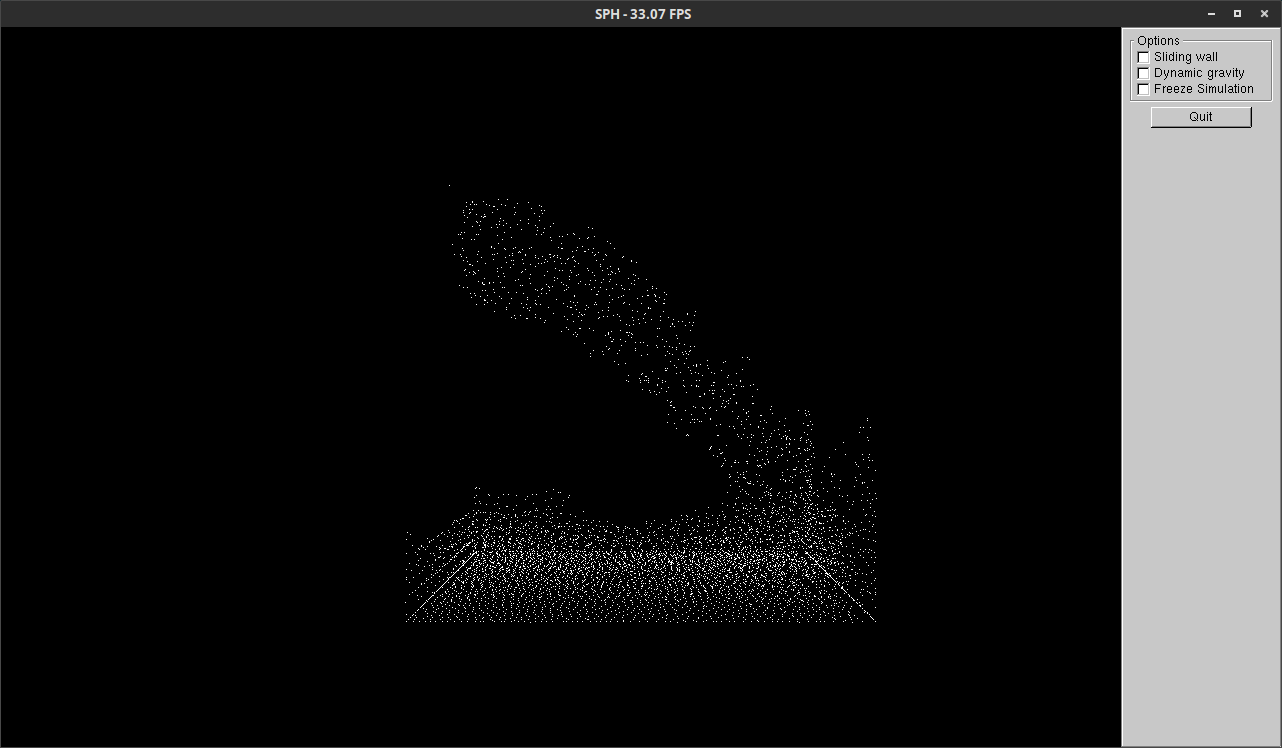
\includegraphics[width=0.48\textwidth,clip=true,trim=10cm 3cm 10cm 3cm]{pictures/sph.png}
\end{center}
\caption{An SPH simulation}
\label{fig:sph} 
\vspace*{2ex}
\hrule
\end{figure}
The visualization part of the definition is the most obvious term for further specification. 
In this context it means that the simulation must end up appearing the same as the fluid in nature.
This means that a fluid has a color, reflects incoming light and refracts light.
The combination of reflection and refraction result in a blending of the fluid with the background.
Moreover, the fluid surface must appear to be smooth.
In nature, this effect is also visible due to surface tension.
It is not a trivial task to quantify the level of realism of a fluid visualization but correct lighting, color, and surface appearance are essential for a realistic fluid visualization.
There are other properties to make a fluid appear realistic such as foam, small surface distortions, and ``thickness'' but do not add as much to the immersion as the aforementioned properties.

The paper by van der Laan et al. \cite{van2009screen} achieves a real-time visualization by a point-splatting approach with a configurable speed-versus-quality trade-off.
They state that this approach is preferable over methods as implicit surface polygonization and other mesh-like constructs due inherent speed limitation.

van der Laan et al. achieve smooth fluid surfaces by applying a sophisticated smoothing method to the point splats which is discussed in detail in section~\ref{sec:smoothing}.

\subsection{Related work}
Various methods are developed that try to achieve a natural rendering of fluid.

A method to render fluids has been proposed by \cite{williams2008fluid} that uses Marching Tiles. 
The method creates smooth surfaces but the drawback is that these surfaces can not be rendered in real-time.

An improvement \cite{rosenberg2008real} proposed is to extract the isosurface to reduce the amount of particles that need to be rendered.
The Marching Cubes algorithm is used as a base for this extraction technique.
The advantage is that rendering becomes relatively fast, however the mesh is not smooth and since it is rendered directly, post-processing the result can not be done.

The problem of both \cite{williams2008fluid} his method and \cite{rosenberg2008real} their method is that they require a fixed grid, which is not desirable for our implementation. 

\cite{muller2007screen} proposed a method where the boundary of a mesh is generated, without the need of a fixed grid.
The surface is smoothed using a binomial filter and creates an intermediate mesh.
The drawback is that this method is computationally very expensive, thus this method can not render fluids in real-time.

\cite{zhang2008adaptive} developed a method that makes use of point-based rendering, therefore a grid is unnecessary.
However, a drawback of this method is that it results in unreasonably thick surfaces.
